\documentclass[a4paper, 12pt]{article}
\usepackage[UTF8]{ctex}
\usepackage{graphicx}
\begin{document}
	\title{第一次实验报告}
	\author{时伟杰}
	\date{2024年8月23日}
	\maketitle
	\tableofcontents
	\newpage
	\pagenumbering{arabic}
	\section{git简介}
	‌‌Git是一个免费的开源分布式版本控制系统‌,旨在快速高效地处理从小型到大型项目的所有事务。它通过记录每次文件的改动,允许同事协作编辑,从而简化了文件管理过程。Git能够自动记录每次文件的改动,使得查看某次改动变得简单,同时支持离线开发,速度和性能优异,特别适合大型项目的多人协作开发。由于其分布式特性、暂存区设计和出色的分支系统,Git能够灵活应对各种工作场景,轻松实现不同工作模式的切换。此外,Git拥有庞大的用户社区和丰富的资源,使得学习和获取帮助变得相对容易。由于其灵活性和受欢迎程度,Git已成为所有团队的绝佳选择,被广泛用于项目管理、代码跟踪和团队协作中。‌
	\section{Latex简介}
	‌LaTeX‌是一种基于ΤΕΧ的排版系统,它利用纯文本格式进行文档排版,即使使用者没有排版和程序设计的知识,也能充分发挥由TeX所提供的强大功能,在几天甚至几小时内生成具有书籍质量的印刷品。LaTeX特别适用于生成高印刷质量的科技和数学类文档,也适用于从简单的信件到完整书籍的所有其他种类的文档。它的优点包括专业排版、数学支持、跨平台性、开源免费、分章节管理和引用管理等功能。LaTeX采用了一种基于标记的方式来创建文档,这种方式允许用户更好地控制文档的排版和格式,与常见的文字处理软件如Microsoft Word不同。LaTeX文档通常包括文档类定义、导言部分(包含设置文档格式、加载宏包和定义自定义命令的内容)、正文部分(包含文档的实际内容,如文字、图像、表格和公式)、章节以及公式和图像的插入。此外,LaTeX提供了功能强大的数学排版功能,支持行内和行间数学公式,以及插入图像并控制其位置和大小。
	
	\section{实例演示与截图}      %方法
	\begin{tabular}[l]{|c|c|c|}   %表格
		\hline
		git操作 &实例       & 介绍    \\
		\hline
		1  & git config --global user.name  & 向git提交姓名 \\
		\hline
		2  & git config --global user.email& 向git提交邮箱 \\
		\hline
		3  & date & 日期 \\
		\hline
		4  & git init & 创建一个本地的项目仓库 \\
		\hline
		5  & git add 123.txt  & 将123.txt提交到暂存区 \\
		\hline
		6  & git commit -m"这是第一次" & 将文件提交到仓库 \\
		\hline
		7  & git log  & 查看提交的节点哈希值以及时间和作者 \\
		\hline
		8 & git log --stat & 比git log多了文件内容变化 \\
		\hline
		9 & git checkout & 代码回溯 \\
		\hline
		10 & git branch & 查看分支 \\
		\hline
		11 & git checkout -b develop & 创建并转化到新建分支 \\
		\hline
		12 & git merge develop& 合并分支 \\
		\hline
		Latex操作 & 实例 &介绍 \\
		\hline
		13 & documentclass & 必须出现在每个LaTeX文档的开头  \\
		\hline
		14 & begin\{documnet\}  &  开头   \\
		\hline
		15 & end\{document\} & 结尾 \\
		\hline
		16 & maketitle & 制作题目 \\
		\hline
		17 & section\{...\} & 节 \\
		\hline
		18 & subsection\{...\} & 小节 \\
		\hline
		19 & chapter\{...\} & 章 \\
		\hline
		20 & label\{labelname\} & 标签 \\
		\hline
		21 & tableofcontents & 创建目录 \\
		\hline
		22 & pagenumbering\{...\} & 页码 \\
		\hline
		23 & newpage & 新建页面 \\
		\hline
		24 & noindent & 段落顶格 \\
		\hline
		25 & enumerate & 有序列表 \\
		\hline
		26 & 百分号 & 注释 \\
		\hline
		27 & 反斜杠   & 特殊字符的转义字符 \\
		\hline
		28 & hline & 插入一个贯穿所有列的横着的分割线 \\
		\hline
		\end{tabular}
		\newpage
		续表:\\
		\begin{tabular}[l]{|c|c|c|}   %表格
		\hline
		29 & begin\{tabular\} end\{tabular\} & 表格 \\
		\hline
		30 & l & 一个左对齐的列 \\
		\hline
		31 & r & 一个右对齐的列 \\
		\hline
		32 & c & 一个向中对齐的列 \\
		\hline
		33 & | & 一个列的竖线 \\
		\hline
		34 & begin\{figure\} end\{figure\} & 图表 \\
		\hline
		35 & centering & 将图片放置在页面的中央 \\
		\hline
		36 & includegraphics\{...\} & 自动将图放置到文档中 \\
		\hline
		37 & begin\{equation\} end\{equation\} & 公式 \\
		\hline
		38 & \^  \_ & 上下标 \\
		\hline
		39 & frac\{numerator\}\{denominator\} & 分数 \\
		\hline
		40 & sqrt\{...\} & 根号 \\
		\hline
		41 & sum & 求和 \\
		\hline
		42 & int & 积分 \\
		\hline
		\end{tabular}
		\section{心得体会}
		Git 是一个分布式版本控制系统,能够高效地管理和记录代码变更。它的分支功能允许你在不影响主线的情况下进行实验和开发。GitHub 作为 Git 的平台,提供了远程存储、代码审查和团队协作的功能。可以使用 pull requests 进行代码审查,通过 issues 跟踪任务和问题。LaTeX 是一个强大的排版系统,特别适合排版数学公式和学术文档。它提供了精确的格式控制和自动化的参考文献管理,能帮助你创建高质量的文档。对于这些工具,实际操作和实践非常重要,使用模板和查阅社区支持也能加速学习进程。\\
		在学习的过程中,也不是一帆风顺的。比如git如果想要在Win11桌面或者其他文件夹运行需要在注册表编辑器上编辑一些参数,经过网上大量的检索和学习才掌握。而且Latex的语法多而杂,在编辑时常常遇到一些问题,查询网上博客才能解决。这些问题也强化了我检索信息和解决问题的能力,提升了我的工作效率和文档质量,让我在技术项目和学术写作中更加得心应手。
		\begin{figure}[h!]
			\centering
			\listoffigures
			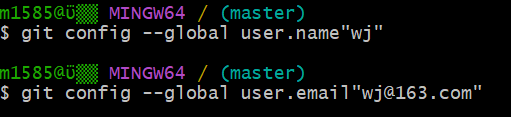
\includegraphics[width=1\textwidth]{1-2}
			\caption{第一和二个实例演示}
			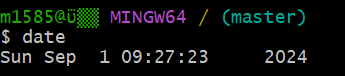
\includegraphics[width=1\textwidth]{3}
			\caption{第三个实例演示}
			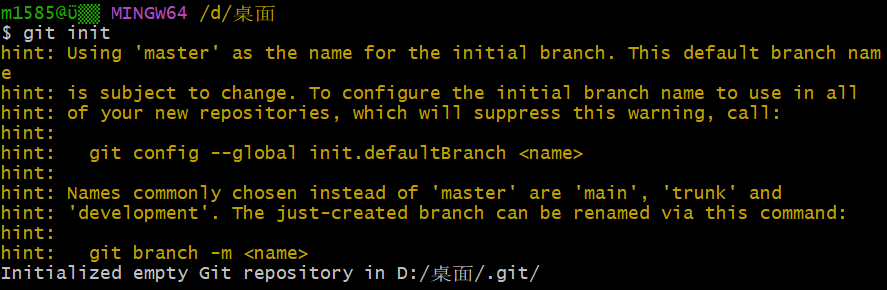
\includegraphics[width=1\textwidth]{4}
			\caption{第四个实例演示}
		\end{figure}
		\begin{figure}[h!]
			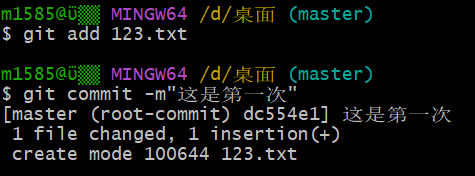
\includegraphics[width=1\textwidth]{5-6}
			\caption{第五和六个实例演示}
			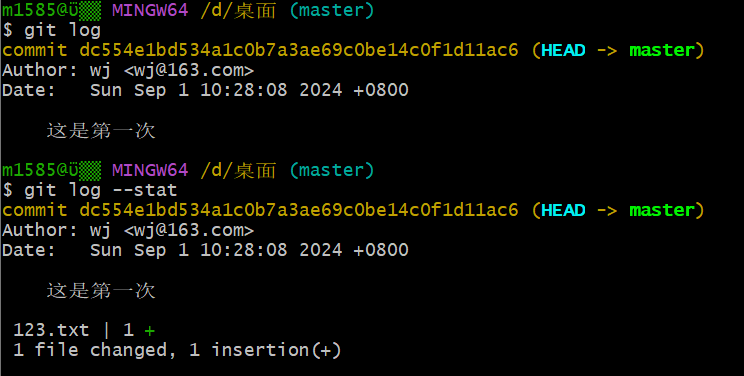
\includegraphics[width=1\textwidth]{7-8}
			\caption{第七和八个实例演示}
			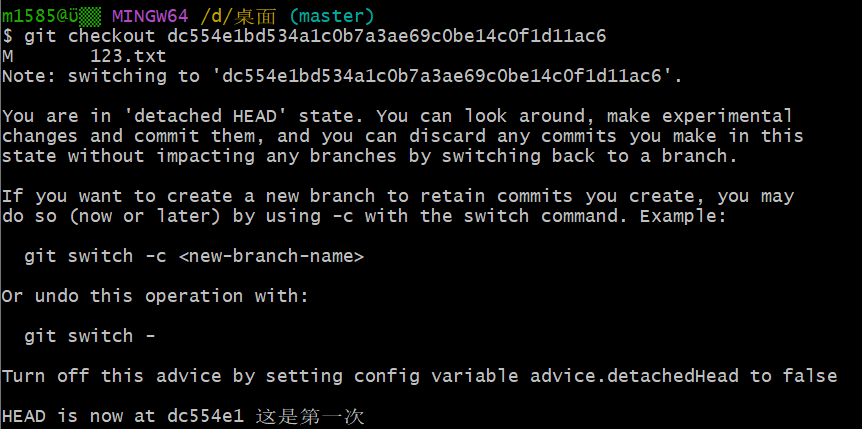
\includegraphics[width=1\textwidth]{9}
			\caption{第九个实例演示}
		\end{figure}
		\begin{figure}[h!]
			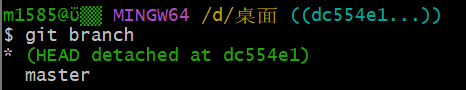
\includegraphics[width=1\textwidth]{10}
			\caption{第十个实例演示}
			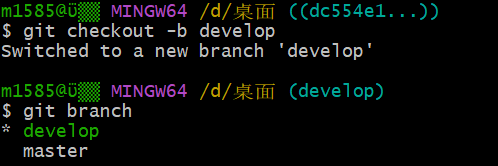
\includegraphics[width=1\textwidth]{11}
			\caption{第十一个实例演示}
			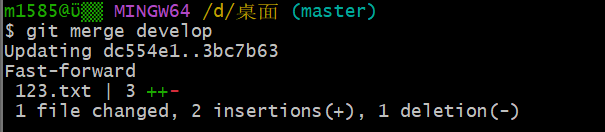
\includegraphics[width=1\textwidth]{12}
			\caption{第十二个实例演示}
		\end{figure}
		
\end{document}